\documentclass[pdflatex,sn-mathphys-num]{sn-jnl}
\usepackage{url}
\usepackage{subcaption}
\usepackage{placeins}
\usepackage{pgfplots}
\pgfplotsset{compat=1.18}
\usepackage[T1]{fontenc}
\usepackage{textcomp}
\usepackage{upquote}
\usepackage{graphicx}%
\usepackage{multirow}%
\usepackage{amsmath,amssymb,amsfonts}%
\usepackage{amsthm}%
\usepackage{xcolor}%
\usepackage{booktabs}%
\usepackage{algorithm}%
\usepackage{algorithmicx}%
\usepackage[noend]{algpseudocode}%
\usepackage{listings}%
\usepackage{tikz}
\usepackage{tabularx}
\usepackage{microtype}
\usepackage[utf8]{inputenc}
\usepackage[english]{babel}
\usepackage{tcolorbox}
\tcbuselibrary{skins, breakable}
\usepackage{enumitem}
\usepackage{pifont}
\usepackage{hyperref}
\usetikzlibrary{arrows.meta,positioning,shapes.geometric,fit,backgrounds,calc}
\hypersetup{colorlinks=true, linkcolor=black, urlcolor=black, citecolor=black}

\theoremstyle{thmstyleone}%
\newtheorem{proposition}{Proposition}%
\theoremstyle{thmstyletwo}%
\newtheorem{example}{Example}%
\theoremstyle{thmstylethree}%
\newtheorem{definition}{Definition}%

\raggedbottom
\renewcommand{\topfraction}{0.92}
\renewcommand{\textfraction}{0.08}
\renewcommand{\floatpagefraction}{0.85}

\newcommand{\cj}{\textsc{Claim2Job}}
\newcommand{\skill}{\texttt{use-hpc}}
\newcommand{\auto}{\textsc{AutoM2M}}
\newcommand{\code}[1]{\texttt{#1}}
\newcommand{\RQ}[1]{\textbf{RQ#1}}
\newcommand{\V}[1]{\textsf{V#1}}
\newcommand{\I}[1]{\textsf{I#1}}
\newcommand{\cmark}{\ding{51}}
\newcommand{\xmark}{\ding{55}}
\algnewcommand{\LineComment}[1]{\State \(\triangleright\) \textit{#1}}

\definecolor{rawbg}{RGB}{255,248,230}
\definecolor{rawbar}{RGB}{214,150,40}
\definecolor{modelbg}{RGB}{235,244,255}
\definecolor{modelbar}{RGB}{60,110,180}
\definecolor{enginebg}{RGB}{236,250,238}
\definecolor{enginebar}{RGB}{60,145,80}
\definecolor{llmbg}{RGB}{248,238,252}
\definecolor{llmbar}{RGB}{140,80,160}

\lstset{frame=l, framerule=2pt, framesep=6pt, xleftmargin=9pt, framexleftmargin=0pt,
        basicstyle=\ttfamily\fontsize{6.8}{7.9}\selectfont, breaklines=false, columns=fullflexible,
        keepspaces=true, showstringspaces=false, numbers=none, upquote=true,
        commentstyle=\itshape\color{black!55}, captionpos=t, float=tbp, aboveskip=6pt, belowskip=4pt,
        backgroundcolor=\color{modelbg}, rulecolor=\color{modelbar}}

\newcommand{\DataStatus}{%
\begin{tcolorbox}[enhanced, breakable, colback=rawbg, colframe=rawbar, boxrule=0.6pt, arc=1pt,
  left=6pt, right=6pt, top=4pt, bottom=4pt]
\small\textbf{Status of the data in this version.} Every number in
Sections~\ref{sec:res-rq1}--\ref{sec:res-rq4} is \emph{measured}. It comes from
the pipeline's own ledgers, from Slurm accounting (\code{sacct}) and from GPU
telemetry of the pilot deployment on the Nibi cluster, or from micro-benchmarks
of the released template. All of it is regenerated by
\code{docs/use-hpc-eval/analyze\_pilot.py} from \code{hpc/logs/} and
\code{sacct\_raw.psv}. Figures for the full \auto{} run are a \emph{snapshot}
taken while the run was in progress (2026-10-13, 13:04 EDT), not its final
totals. The multi-repository study of Section~\ref{sec:res-rq5} is
\emph{pre-registered}: its protocol is fixed, but its results are pending and
are marked as such. No number in this paper is simulated.
% TODO(author): replace the snapshot by final totals and fill Table~\ref{tab:repos} when the study completes.
\end{tcolorbox}}

\begin{document}

\title[Every Claim a Job]{Every Claim a Job: Compiling Research Papers into Contract-Checked, Self-Auditing GPU Pipelines on HPC Clusters}

\author*[1]{\fnm{Majid} \sur{Babaei}}\email{ai4se4ai@gmail.com}
\affil*[1]{\orgname{ai4se4ai-lab}}
% TODO(author): complete affiliations and co-authors.

\abstract{\textbf{Context.} A paper's results are only as authentic as the
runs behind them. Yet the step from a paper's experimental design to thousands
of GPU jobs on a shared cluster is still done by hand. Scripts are written ad
hoc; failed jobs, silent CPU fallbacks and half-finished grids go unnoticed;
and the link from a claim in the paper to the run that supports it is lost.
LLM coding agents can now write such scripts, but an improvising agent on a
shared supercomputer is a liability rather than a help.
\textbf{Objective.} We present \cj{}, an approach that \emph{compiles} a
paper's experimental claims into a typed experiment graph. It executes that
graph as a contract-checked, GPU-only, self-auditing Slurm pipeline. We
implement it as \skill{}, an open-source agent skill for Claude Code.
\textbf{Method.} An LLM agent reads the paper and the code and proposes an
experiment inventory and a graph of stages, matrices, dependencies and data
contracts. Deterministic programs then decide. A validator checks six
well-formedness conditions before anything is submitted. Runtime guards enforce
four execution invariants: no computation on login nodes, a GPU behind every
job, idempotent resumption, and requeue before the time limit. A smoke
projection runs every stage and every edge of the graph at minimal size, a live
audit reports every job, step and record, and a collector turns raw outputs into
CSVs, tables, figures and a coverage matrix from each claim to the job that
supports it.
\textbf{Results.} In a pilot deployment that runs the 44{,}352-run evaluation
of a software-engineering paper on the Nibi cluster (26 jobs, 122 steps, up to
2~H100 GPUs per job), all three smoke runs completed 36/36 steps on 7--8 GPU
nodes in 18--24 minutes. That is 2.0--2.7$\times$ faster than serial
execution. Three failed setup gates cancelled all 75 dependent jobs before they
started, at a cost of at most 0.27 GPU-hours each. The full run sustained a mean concurrency of 14.6 jobs over its first 3.1 hours, and GPU telemetry
exposed two matrix jobs running at 2--5\% GPU utilisation while the other 12
averaged 73\%. The machinery is cheap: 7\,ms per step, 0.5\,s for a 5{,}000-cell
audit, and 1.4\,s to collect 100{,}000 records.
\textbf{Conclusion.} Treating every claim as a job, and every job as something
a program checks, makes large-scale experiments on HPC both faster to run and
easier to trust. A pre-registered study on independent GitHub repositories will
test how far the approach generalises.}

\keywords{Reproducibility, High-performance computing, Slurm, GPU, Experiment
management, LLM agents, Agent skills, Research software engineering}

\maketitle

% =========================================================================
\section{Introduction}\label{sec:intro}

A scientific paper is a set of \emph{claims} backed by \emph{runs}. Behind a
sentence such as ``the checker detects 96\% of seeded defects'' or a table of
success rates over seven models and three seeds stand thousands of executions
of research code. Whether the claim is authentic depends on whether those
executions happened as described, completed, and were aggregated without
loss. The record is not reassuring. Most researchers report having failed to
reproduce others' results~\cite{baker2016reproducibility}. Much published
systems and AI research cannot even be rebuilt or rerun from its
artefacts~\cite{collberg2016repeatability,gundersen2018state}. Most research
code deposited in repositories does not execute
cleanly~\cite{trisovic2022large,pimentel2019large}.

Modern experiments add a second gap: \emph{scale}. A software-engineering study
of LLM agents may compare eight conditions on seven models, 264 tasks and three
seeds, which is 44{,}352 runs and thousands of GPU-hours. Such studies must run
on shared HPC clusters, where the scheduler is unforgiving.
\begin{itemize}[leftmargin=1.4em, itemsep=1pt]
\item Work started on a login node harms hundreds of other users.
\item A job that silently falls back to the CPU burns its allocation.
\item A downstream job that starts on missing inputs produces plausible
garbage.
\item A 24-hour time limit cuts a grid in half without anyone noticing.
\end{itemize}
The researcher's view of the experiment, ``the table in Section 5'', and the
cluster's view, ``job 23880896 is RUNNING on g21'', are disconnected.

LLM coding agents~\cite{yang2024sweagent,wang2025openhands} can write Slurm
scripts in seconds, and agent benchmarks now test whether agents can set up and
reproduce research
repositories~\cite{bogin2024super,siegel2024corebench,starace2025paperbench}.
But an agent that \emph{improvises} on a shared supercomputer is exactly what
cluster operators fear. It may poll the scheduler in a tight loop, install
packages on the login node, request the wrong GPUs, or declare success after
the first job finishes. The question is not whether an agent can write
\code{sbatch} files. It is how to make the agent's output \emph{checkable}.

\paragraph{Key insight} We treat the paper itself as the specification of a
program. Each experimental claim becomes a node or step of an
\emph{experiment graph} with typed resources, explicit dependencies and
declared data contracts. The LLM \emph{proposes} this graph, and deterministic
programs \emph{decide}:
\begin{itemize}[leftmargin=1.4em, itemsep=1pt]
\item a validator checks the graph before submission;
\item runtime guards enforce invariants inside every job;
\item the scheduler's dependency semantics order the work;
\item an audit and a collector report what actually happened, claim by claim.
\end{itemize}
The principle is ``LLMs propose; programs decide'', the same one that
underlies checked LLM agent teams. Here we apply it to the experimental
apparatus itself.

\paragraph{This paper} We present \cj{} and its implementation \skill{}, an
agent skill~\cite{anthropic2025skills} that installs with one command and ships
a tested pipeline template of about 1{,}560 lines of Python and Bash. We make
the following contributions.
\begin{enumerate}[label=\textbf{C\arabic*}, leftmargin=2.2em, itemsep=1pt]
\item \emph{A claim-to-job model} of experiments on HPC: the experiment
inventory, the experiment graph with matrix cells and three dependency kinds,
data contracts, and a coverage matrix that links every claim of a paper to the
job and file that support it (Section~\ref{sec:approach}).
\item \emph{Six well-formedness conditions} (\V{1}--\V{6}) checked before
submission, \emph{four execution invariants} (\I{1}--\I{4}) enforced inside
jobs, and a \emph{smoke projection} that exercises every stage and every edge
of the graph at minimal cost.
\item \emph{An agent skill}, \skill{}, that guides a coding agent through
inventory, scaffolding, configuration, verification, execution and
documentation, and confines its freedom to a validated configuration file.
\item \emph{An evaluation} on a 44{,}352-run pilot study using Slurm
accounting, the pipeline's ledgers and GPU telemetry, micro-benchmarks of the
machinery, and a pre-registered protocol for a multi-repository study
(Section~\ref{sec:eval}).
\end{enumerate}

\DataStatus

% =========================================================================
\section{Background}\label{sec:background}

\subsection{Reproducibility of computational research}\label{sec:bg-repro}

Computational reproducibility has many names: repeatability (same team, same
set-up), reproducibility (different team, same artefacts) and replicability
(different team, new
artefacts)~\cite{acm2020badges,vitek2011repeatability}. Community responses
include:
\begin{itemize}[leftmargin=1.4em, itemsep=1pt]
\item artefact evaluation and badges~\cite{acm2020badges};
\item reproducibility checklists~\cite{pineau2021improving};
\item data principles~\cite{wilkinson2016fair};
\item recommendations for publishing code, data and
workflows~\cite{stodden2016enhancing};
\item tools that capture execution environments, such as ReproZip and
containers~\cite{chirigati2016reprozip,kurtzer2017singularity}.
\end{itemize}
These help a second team rerun a \emph{small} computation. They say little
about the experiment as a whole: which runs a claim needs, whether all of them
completed, and how their outputs became the paper's tables. For performance
claims, Hoefler and Belli list how incomplete reporting misleads
readers~\cite{hoefler2015scientific}. We take the same view for the whole
experimental pipeline.

\subsection{Batch scheduling on HPC clusters}\label{sec:bg-slurm}

Slurm~\cite{yoo2003slurm} is the dominant workload manager on academic
clusters. The concepts \cj{} builds on are listed below.
\begin{description}[leftmargin=1.1em, style=nextline, itemsep=1pt]
\item[Jobs and resources] \code{sbatch} queues a batch script with requested
resources: time, CPUs, memory and generic resources such as GPUs. A
fair-share scheduler decides when it starts. Login nodes are shared and are
meant only for editing and submission.
\item[Job arrays] \code{--array=0-N\%K} queues $N{+}1$ tasks of one script with
one call, at most $K$ of them at a time. Each task sees its index in
\code{SLURM\_ARRAY\_TASK\_ID}.
\item[Dependencies] \code{--dependency=afterok:J} starts a job only after job
(or array) $J$ succeeded; \code{afterany} waits for any ending; \code{aftercorr}
starts array task $i$ after task $i$ of the upstream array succeeded. With
\code{--kill-on-invalid-dep=yes}, a dependency that can never be satisfied
cancels the job.
\item[Signals and requeue] \code{--signal=B:USR1@900} sends a signal to the
batch shell 900\,s before the time limit, and \code{scontrol requeue} puts a
job back in the queue under the same ID.
\item[GPU partitioning] Multi-Instance GPU (MIG) splits an H100 into isolated
slices, for example \code{h100\_1g.10gb}, one eighth of a GPU~\cite{nvidia2023mig}.
\end{description}
Cluster operators add rules of conduct: no heavy work on login nodes, no tight
polling of the scheduler, no \code{sleep} inside jobs, packages from a curated
wheelhouse, and active work on purged scratch storage with results kept on
backed-up project storage~\cite{alliance2026docs}.

\subsection{Workflow management systems}\label{sec:bg-wms}

Scientific workflow systems such as Pegasus~\cite{deelman2015pegasus},
Snakemake~\cite{molder2021snakemake}, Nextflow~\cite{ditommaso2017nextflow},
Parsl~\cite{babuji2019parsl} and FireWorks~\cite{jain2015fireworks} describe
computations as graphs of tasks and submit them to schedulers. They are
powerful, general and mature. They also bring their own language, runtime and
mental model. They describe \emph{how} to compute, not \emph{which claims} the
computation supports. \cj{} is deliberately thinner: a JSON graph, plain Slurm
primitives, and an audit that a reviewer can read. Its additions are the link
to the paper, the guardrails for an agent author, and the smoke projection.

\subsection{LLM coding agents and agent skills}\label{sec:bg-agents}

Coding agents run an LLM in a loop with tools (shell, editor, tests) and solve
repository-level tasks~\cite{jimenez2024swebench,yang2024sweagent,wang2025openhands}.
Benchmarks now ask whether agents can set up research repositories
(SUPER~\cite{bogin2024super}), reproduce published computational results
(CORE-Bench~\cite{siegel2024corebench}), or replicate whole papers
(PaperBench~\cite{starace2025paperbench}). These benchmarks measure the
\emph{agent}. We contribute the \emph{apparatus} an agent should use when the
target is a shared cluster. An \emph{agent skill}~\cite{anthropic2025skills} is
a folder of instructions, reference documents and scripts that an agent loads
on demand. Only its name and a short description stay in context until it is
needed. A skill is thus a natural carrier for a method: it tells the agent what
to do, and ships the programs that check that it was done.

\subsection{Running example}\label{sec:example}

Our running example is the evaluation of \auto{}, an approach that checks
LLM-assembled agent teams. Its paper asks four research questions:
\begin{itemize}[leftmargin=1.4em, itemsep=1pt]
\item RQ1: diagnosis, by coding failures;
\item RQ2: prevention, by mutation analysis, seeded defects and LLM critics;
\item RQ3: effect, by an 8-condition $\times$ 7-model $\times$ 264-task
$\times$ 3-seed matrix;
\item RQ4: attribution and repair, by fault injection and transcript baselines.
\end{itemize}
It needs seven open-weight models served by an inference server on H100 GPUs,
two benchmarks, a corpus of annotated failures, and an analysis that produces
every table and figure. It is a demanding, realistic target: heterogeneous
stages, auxiliary models that must share a GPU, hard dependencies (studies that
consume the matrix's output), and days of GPU time.

% =========================================================================
\section{Approach}\label{sec:approach}

\subsection{Overview}\label{sec:overview}

Figure~\ref{fig:overview} shows \cj{} end to end. Two inputs, the
\emph{document} (paper, report or design document) and the \emph{source code},
pass through six phases. In each phase the agent (purple) proposes, and a
program (green) decides or records.

\begin{figure}[t]
\centering
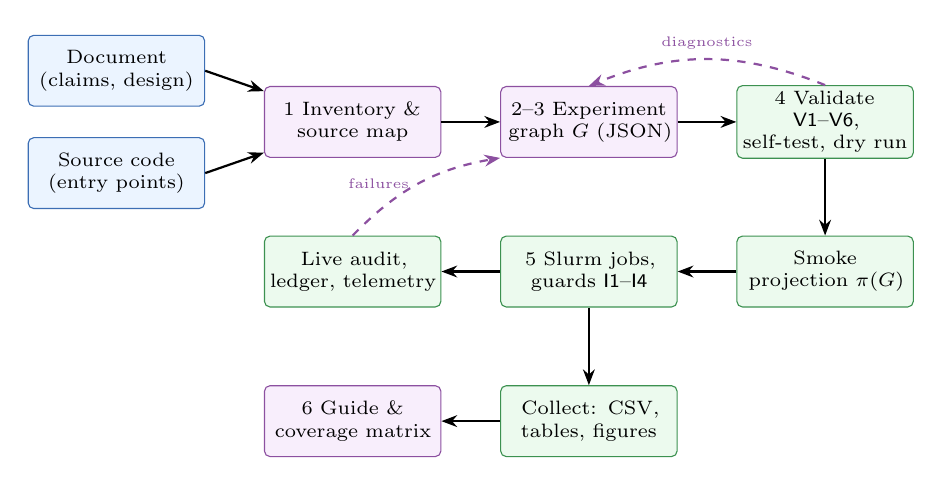
\begin{tikzpicture}[font=\scriptsize,
  box/.style={draw, rounded corners=2pt, align=center, minimum height=9mm, text width=21mm, inner sep=2pt},
  llm/.style={box, fill=llmbg, draw=llmbar},
  prog/.style={box, fill=enginebg, draw=enginebar},
  data/.style={box, fill=modelbg, draw=modelbar},
  arr/.style={-{Stealth[length=2mm]}, thick}]
\node[data] (doc) at (0,0.65) {Document\\(claims, design)};
\node[data] (src) at (0,-0.65) {Source code\\(entry points)};
\node[llm]  (inv)   at (3.0,0) {1 Inventory \&\\source map};
\node[llm]  (graph) at (6.0,0) {2--3 Experiment\\graph $G$ (JSON)};
\node[prog] (val)   at (9.0,0) {4 Validate \V{1}--\V{6},\\self-test, dry run};
\node[prog] (smoke) at (9.0,-1.9) {Smoke\\projection $\pi(G)$};
\node[prog] (run)   at (6.0,-1.9) {5 Slurm jobs,\\guards \I{1}--\I{4}};
\node[prog] (audit) at (3.0,-1.9) {Live audit,\\ledger, telemetry};
\node[prog] (coll)  at (6.0,-3.8) {Collect: CSV,\\tables, figures};
\node[llm]  (guide) at (3.0,-3.8) {6 Guide \&\\coverage matrix};
\draw[arr] (doc.east) -- (inv); \draw[arr] (src.east) -- (inv);
\draw[arr] (inv) -- (graph); \draw[arr] (graph) -- (val);
\draw[arr] (val) -- (smoke); \draw[arr] (smoke) -- (run);
\draw[arr] (run) -- (audit); \draw[arr] (run) -- (coll); \draw[arr] (coll) -- (guide);
\draw[arr, dashed, llmbar] (val.north) to[bend right=22] node[above, font=\tiny]{diagnostics} (graph.north);
\draw[arr, dashed, llmbar] (audit.north) to[bend left=18] node[left, font=\tiny]{failures} (graph.south west);
\end{tikzpicture}
\caption{\cj{} at a glance. Purple: the agent proposes. Green: programs check,
run and record. Blue: inputs. Validator diagnostics and audited failures flow
back to the agent, which revises the graph, never the guards.}
\label{fig:overview}
\end{figure}

\begin{enumerate}[leftmargin=1.4em, itemsep=1pt]
\item \emph{Inventory.} The agent extracts the experimental claims and design
of the document, and maps each to source entry points.
\item \emph{Scaffold.} A script copies the pipeline template into
\code{hpc/}.
\item \emph{Configure.} The agent writes the experiment graph $G$ as a JSON
file, plus site settings.
\item \emph{Verify.} The validator checks $G$. A dry run shows the exact
\code{sbatch} commands, and the smoke projection $\pi(G)$ runs every stage on
real GPU nodes.
\item \emph{Execute.} $G$ is submitted. Guards inside every job enforce the
invariants, the audit reports progress, and the collector produces results.
\item \emph{Document.} The agent writes a guide whose centrepiece is the
coverage matrix from claims to jobs to outputs.
\end{enumerate}

\subsection{Experiment inventory and claims}\label{sec:inventory}

\begin{definition}[Claim]\label{def:claim}
A \emph{claim} $c=(q,m,a,r)$ of a document consists of a research question or
hypothesis $q$, a metric $m$ computed over runs, the artefact $a$ (table,
figure or sentence) that reports it, and an optional decision rule $r$, a
predicate on $m$ such as ``the lower bound of the 95\% interval exceeds 20\%''.
\end{definition}

The \emph{experiment inventory} lists, besides the claims:
\begin{itemize}[leftmargin=1.4em, itemsep=1pt]
\item the \emph{subjects} (datasets, benchmarks, and what is hidden from the
system under test);
\item the \emph{factors} (conditions, models, seeds and hyper-parameters) and
the design size they multiply to;
\item \emph{side studies} and \emph{auxiliary roles} (judges, coders, critics);
\item \emph{statistics} and the units of analysis;
\item \emph{fixed parameters};
\item \emph{stated gaps} (the document's own TODOs and threats).
\end{itemize}
The agent cites document labels for every row. When the document and the code
disagree, the agent must ask the human which one wins, and not resolve it
silently.

\subsection{The experiment graph}\label{sec:graph}

\begin{definition}[Experiment graph]\label{def:graph}
An experiment graph is $G=(S,\prec,E,\mathit{cells},\sigma,\rho)$ where
\begin{itemize}[leftmargin=1.4em, itemsep=1pt]
\item $S$ is a finite set of \emph{stages}, totally ordered by submission
order $\prec$;
\item $E\subseteq S\times S\times\{\mathit{ok},\mathit{any},\mathit{corr},\mathit{notok}\}$
contains a \emph{dependency} $(s',s,k)$ only if $s'\prec s$;
\item $\mathit{cells}(s)=\prod_{p\in P_s} D_p$ is the Cartesian product of the
stage's \emph{matrix} parameters, kept in a fixed order. A stage without a
matrix has one empty cell;
\item $\sigma(s)=\langle t_1,\dots,t_n\rangle$ is the ordered list of
\emph{steps}, each a command template or a built-in action;
\item $\rho(s)$ are the stage's \emph{resources}: GPU kind and count (whole or
MIG slice), nodes, tasks, CPUs, memory, time limit and requeue flag.
\end{itemize}
\end{definition}

Every stage becomes one \code{sbatch} submission. A stage with more than one
cell becomes a job array, with cell $i$ as array task $i$. Every dependency
becomes a Slurm dependency on the upstream job ID with the matching type, plus
\code{--kill-on-invalid-dep=yes}. The three dependency kinds encode three
experimental roles:
\begin{itemize}[leftmargin=1.4em, itemsep=1pt]
\item $\mathit{ok}$ for \emph{gates}: setup, data and model verification, and a
pre-flight run. Nothing should start unless the gate passed.
\item $\mathit{any}$ for \emph{consumers of partial data}: analysis and
collection. One failed cell must not block the study.
\item $\mathit{corr}$ for \emph{cell-wise pipelining}: post-processing of cell
$i$ starts as soon as cell $i$ succeeds.
\end{itemize}
A command template is filled from the graph's variables, the cell's parameter
values and built-ins: the results root $R$, the run ID, the cell key, and the
node and task counts.

\paragraph{Data contracts} Each step $t$ declares path patterns
$N(t)$ (\emph{needs}) and $P(t)$ (\emph{produces}), relative to the run's
results root $R$ and instantiated per cell. Before $t$ runs, every pattern in
$N(t)$ must match at least one file, or $t$ fails with ``missing input''. After
$t$ exits successfully, every pattern in $P(t)$ must match, or $t$ fails with
``declared output missing''. Contracts are the \emph{connection} between stages:
the scheduler orders the jobs, and the contracts check that the hand-off
actually happened. In the spirit of design by contract~\cite{meyer1992dbc}, a
violated contract stops the step at the boundary where the fault is visible.
It never lets the fault surface three stages later as a strange number in a
table.

\paragraph{Results specification} $G$ also states how raw outputs become
results:
\begin{itemize}[leftmargin=1.4em, itemsep=1pt]
\item \emph{tables}: glob patterns whose CSV or JSON-lines files are
concatenated and flattened;
\item \emph{summaries}: group-by keys and aggregations (mean, median, rate,
std, \dots);
\item \emph{plots}: bar, line, scatter or box;
\item files to \emph{copy} and directories to \emph{archive}.
\end{itemize}

\subsection{Well-formedness: what is checked before submission}\label{sec:validate}

The validator runs on the login node in under a second. It evaluates six
conditions on $G$ alone, before any GPU is requested.
\begin{description}[leftmargin=1.1em, style=nextline, itemsep=1pt]
\item[\V{1} Identity] Stage names are unique and safe as file and job names,
and step names are unique within a stage.
\item[\V{2} Order] Every dependency refers to an existing, \emph{earlier}
stage. $(S,E)$ is therefore acyclic by construction, and submission in $\prec$
order always has the upstream job IDs at hand.
\item[\V{3} Correspondence] For every $(s',s,\mathit{corr})\in E$,
$|\mathit{cells}(s)|=|\mathit{cells}(s')|$, and $s$ inherits the cells of $s'$
(\code{matrix\_from}), so task $i$ means the same cell in both arrays.
\item[\V{4} GPU policy] Every stage requests a GPU or MIG slice unless it is
explicitly marked CPU-only. A stage cannot reach the CPU by omission.
\item[\V{5} Closure] Every placeholder of every command, need and product of
every cell resolves. The self-test instantiates all of them for the full and
for the smoke graph.
\item[\V{6} Executability] Every step has a command or a known built-in, and
the dry run builds an \code{sbatch} command for every stage.
\end{description}

\subsection{Execution invariants: what is enforced inside jobs}\label{sec:invariants}

All stages share one batch script and one step runner (Algorithm~\ref{alg:runner}).
The batch script enforces four invariants.

\begin{description}[leftmargin=1.1em, style=nextline, itemsep=1pt]
\item[\I{1} No computation on login nodes] The step runner refuses to execute
unless it runs inside a Slurm allocation (exit code 10). The submitter and the
audit only read and write small files and call \code{sbatch}, \code{squeue} and
\code{sacct} once each per action.
\item[\I{2} A GPU behind every job] The batch script exits with code 5 if no GPU
is visible (\code{CUDA\_VISIBLE\_DEVICES} empty or \code{nvidia-smi -L}
failing). A stage that expects a GPU never silently computes on the CPU. A
sampler records utilisation, memory and power every 60\,s for the audit.
\item[\I{3} Idempotent resumption] Each step leaves a completion marker, and a
restarted job skips marked steps. Long commands follow an
\emph{append-and-skip} discipline: one record per finished unit of work, and
units already recorded are skipped on restart.
\item[\I{4} Requeue before the limit] Long stages request
\code{--signal=B:USR1@900} and \code{--requeue}. On the signal, the job stops
its children and services cleanly, records the event, and calls
\code{scontrol requeue} on itself (or on its array task), up to a cap. It reads
the true restart count from the scheduler, because the environment variable is
not always updated after a requeue.
\end{description}

\begin{algorithm}[t]
\caption{Step runner for one cell $c$ of stage $s$ (inside a job).}\label{alg:runner}
\begin{algorithmic}[1]
\Require frozen graph $G$, results root $R$, ledger $L$
\If{not inside a Slurm allocation} \Return 10 \Comment{\I{1}}\EndIf
\State $\kappa \gets$ context(vars, $c$, built-ins);\quad $F\gets\emptyset$
\For{$t \in \sigma(s)$}
  \If{marker($s,c,t$) exists and not $t.\mathit{always}$} \textbf{continue} \Comment{\I{3}}\EndIf
  \State write running-marker($s,c,t$) \Comment{read by the live audit}
  \If{$\exists n\in N(t)$: glob($R$, fill($n,\kappa$)) $=\emptyset$} $rc\gets 6$ \Comment{missing input}
  \Else
    \For{attempt $=0..t.\mathit{retries}$} \State $rc\gets$ execute(fill($t,\kappa$)) \Comment{bash, or \code{srun} on all tasks}
      \If{$rc=0$} \textbf{break} \EndIf \EndFor
    \If{$rc=0 \wedge \exists p\in P(t)$: glob($R$, fill($p,\kappa$)) $=\emptyset$} $rc\gets 7$ \Comment{output missing} \EndIf
  \EndIf
  \State append $(\mathit{job},\mathit{task},\mathit{restart},s,c,t,\mathit{start},\mathit{end},rc,\mathit{note},\mathit{cmd})$ to $L$
  \If{$rc=0$} write marker($s,c,t$) \Else{} $F\gets F\cup\{t\}$; \textbf{if} $t.\mathit{critical}$ \textbf{then break} \EndIf
\EndFor
\State \Return $[F=\emptyset\,?\,0:1]$
\end{algorithmic}
\end{algorithm}

\begin{proposition}[Resumption]\label{prop:resume}
Let every non-\emph{always} step of a cell be append-and-skip. If the job of
the cell is interrupted at any point and restarted any number of times, the
set of completed records after the final, uninterrupted execution equals the
set produced by one uninterrupted execution. No step whose marker exists is
executed again.
\end{proposition}
\noindent\emph{Argument.} Markers are written only after a step returned 0 and
its products exist, so a marked step is complete. An unmarked step is
re-executed. Its command skips every record already present and recomputes
only missing ones. The final execution therefore completes exactly the
complement of what earlier attempts completed. Two caveats apply: records of
stochastic computations are not re-drawn, so their values depend on the
interruption point, not the set; and a partially written last record must be
skipped as unparseable. \hfill$\square$

\begin{proposition}[Gate soundness]\label{prop:gate}
If cell $i$ of stage $s$ fails, then no cell that depends on it starts on that
run's data. A cell depends on it through a path of dependencies in which every
$\mathit{ok}$ edge involves all cells of its upstream stage, and every
$\mathit{corr}$ edge involves only the corresponding cell.
\end{proposition}
\noindent\emph{Argument.} By the semantics of \code{afterok} and
\code{aftercorr}, the dependent never becomes eligible. With Slurm's
kill-on-invalid-dependency option it is cancelled, and cancellation propagates
transitively. Section~\ref{sec:res-rq2}
observes this on real failures. \hfill$\square$

\subsection{The smoke projection}\label{sec:smoke}

A full run may take days. A configuration error in its last stage should cost
minutes, not days. The \emph{smoke projection} $\pi(G)$ keeps every stage,
every dependency and every step of $G$, but:
\begin{itemize}[leftmargin=1.4em, itemsep=1pt]
\item replaces the variables by small sizes (tasks, seeds, items);
\item keeps the first $k$ cells of every matrix;
\item replaces every time limit by a short one.
\end{itemize}
Because $\pi$ preserves $(S,E,\sigma)$, a successful smoke run has executed
every step of every stage at least once, through every dependency kind and
every data contract, on real GPU nodes, with the real module stack, wheels,
services and collector. This is \emph{structural coverage} of the pipeline,
the analogue of statement and branch coverage for the experimental apparatus.
Smoke runs carry their own run-ID prefix, and their collected summary is
labelled as not for reporting.

\subsection{Auditing: from scheduler states to claims}\label{sec:audit}

\cj{} records nine levels of evidence (Table~\ref{tab:audit}). The \emph{live
audit} joins the scheduler's view and the pipeline's view into one table, with
one row per stage $\times$ cell (Figure~\ref{fig:audit}). The scheduler's view
comes from one \code{squeue} and one \code{sacct} call per snapshot. The
pipeline's view comes from the ledger, the running markers, the step logs and
the progress files. Each row shows:
\begin{itemize}[leftmargin=1.4em, itemsep=1pt]
\item the state, node, and run time against the limit;
\item the queue reason;
\item steps done out of the total, and a progress bar of records written
against records expected;
\item the current or failed step.
\end{itemize}
Every failed step is listed with its reason, the relevant log lines and the
log path. Snapshots are saved, so the audit is itself part of the record. The
refresh interval is bounded below by 60\,s, and watch mode ends by itself when
no job is pending or running. Monitoring cannot turn into a polling loop
against the scheduler.

\begin{table}[t]
\centering\small
\caption{Audit levels and the evidence \cj{} keeps for each.}\label{tab:audit}
\begin{tabularx}{\textwidth}{@{}l X X@{}}
\toprule
Level & Question & Evidence \\
\midrule
Intent & What was supposed to run? & frozen configuration; graph with cells expanded \\
Code identity & Which code produced the results? & run manifest: commit, dirty files, diff hash, content hashes \\
Environment & With what software and hardware? & module list, \code{pip freeze}, GPU inventory, model digests \\
Gates & Were the inputs sane before GPU-days were spent? & critical setup steps, pre-flight outputs \\
Jobs & Where, how long, and how did each job end? & Slurm accounting, job and ending ledgers, job logs \\
Steps & Did every step run, and why did it fail? & step ledger (every attempt), step logs, contract notes \\
Data & How far is each cell? & progress specifications, record counts, completeness table \\
Resources & Was the GPU used well? & 60\,s GPU samples, utilisation summary \\
Results & Is every planned output present? & collected summary, coverage matrix in the guide \\
\bottomrule
\end{tabularx}
\end{table}

\begin{figure}[t]
\centering
\begin{lstlisting}
 cells  [OK] 4   [PARTIAL] 2   (total 6)      steps 6/8 ok, 2 failed      records [####################] 100% 24/24

    STAGE[cell]  CELL                STATE    GPU             NODE  RUN / LIMIT    STEPS  PROGRESS                CURRENT/FAILED
 v  main[0]      model=a,dataset=d1  OK       h100:1          g21   0h41m / 1d00h  1/1    [##########] 100% 12/12  -
 ~  followup[0]  model=a,dataset=d1  PARTIAL  h100:1          g26   0h03m / 8h00m  1/2    -                        will_fail
 v  collect[0]   -                   OK       h100_1g.10gb:1  g3    0h01m / 2h00m  1/1    -                        -
 Failures (2)
  x followup[0] will_fail  rc=3
      | Traceback: boom
      log: hpc/logs/<RUN_ID>/steps/followup/a__d1/will_fail.log
\end{lstlisting}
\caption{Excerpt of the live audit from a test run of the template, in ASCII
(the terminal shows coloured state symbols and Unicode progress bars). Node
names and times are illustrative.}
\label{fig:audit}
\end{figure}

\subsection{Collecting results and closing the loop to claims}\label{sec:collect}

The final stage depends on all others with $\mathit{any}$. It runs the
project's own analysis (statistical tests, the paper's exact tables) and then
the built-in collector. The collector produces:
\begin{itemize}[leftmargin=1.4em, itemsep=1pt]
\item one CSV per table;
\item summaries as CSV, Markdown and booktabs \LaTeX;
\item figures as PNG and PDF;
\item the pipeline records as CSV: every step attempt, job endings,
completeness per cell, and GPU utilisation per job;
\item the run manifest.
\end{itemize}
Directories of many small files are packed into a single archive, and
everything is copied from purged scratch storage to backed-up project storage.

\begin{definition}[Coverage matrix]\label{def:coverage}
For a document with claims $C$ and a graph $G$, the coverage matrix maps each
$c\in C$ to a set of pairs $(t,f)$ of steps and output files such that $f\in
P(t)$ and the metric of $c$ is computed from $f$, together with the collected
file and the artefact $a$ of $c$. $G$ \emph{covers} the document if every claim
has a non-empty entry. Claims without one are listed explicitly as \emph{not
covered}, with a reason.
\end{definition}

The coverage matrix is the bridge from ``the scheduler ran job 23880896'' to
``Table 8 of the paper is supported by these 14 array tasks, whose completeness
is 100\%''. It is written by the agent and checked by a reviewer. Every file it
names exists in the collected results.

\subsection{The agent skill: proposing within guardrails}\label{sec:skill}

\skill{} packages the method as an agent skill: an instruction file, five
reference documents (from paper to experiments; graph schema; Slurm and GPU
usage; audit and results; site notes), a scaffold script, and the pipeline
template. Its description makes the agent load it whenever a user asks to run,
reproduce or scale experiments on a cluster. Its instructions:
\begin{itemize}[leftmargin=1.4em, itemsep=1pt]
\item prescribe the six phases;
\item forbid heavy work on login nodes;
\item require the user's consent before any submission beyond a dry run;
\item tell the agent to summarise one audit snapshot when asked about
progress, instead of polling.
\end{itemize}
The \emph{division of labour} is the core design decision. The agent writes
only the configuration (graph, site settings, requirements, optional service
hooks), the guide, and minimal source edits (redirecting output paths and
making long loops append-and-skip), each of which it must explain. The guards,
the runner, the audit and the collector are fixed, tested code. The agent's
errors therefore surface as validator diagnostics, contract failures or audit
rows, which the agent reads and fixes. They do not surface as wrong numbers.
\skill{} installs on any machine with one command, as a Claude Code plugin from
its public repository~\cite{usehpc2026repo}.

% =========================================================================
\section{Related Work}\label{sec:related}

\paragraph{Workflow management systems} Pegasus~\cite{deelman2015pegasus},
Snakemake~\cite{molder2021snakemake}, Nextflow~\cite{ditommaso2017nextflow},
Parsl~\cite{babuji2019parsl} and FireWorks~\cite{jain2015fireworks} offer rich
graph languages, provenance and executors for many schedulers. \cj{} borrows
their core abstraction, a task graph with data dependencies, but differs in
three ways:
\begin{itemize}[leftmargin=1.4em, itemsep=1pt]
\item its graph is derived from, and traced back to, the claims of a document;
\item it targets an agent author, so its language is a small JSON schema with
a validator rather than a programming language;
\item it compiles to plain Slurm primitives (arrays, dependencies, signals),
which cluster staff can read and support.
\end{itemize}
A \cj{} step can itself invoke a Snakemake or Nextflow workflow.

\paragraph{Reproducibility infrastructure} Environment capture (ReproZip,
containers)~\cite{chirigati2016reprozip,kurtzer2017singularity}, artefact
badges~\cite{acm2020badges} and checklists~\cite{pineau2021improving} make a
computation \emph{rerunnable}. \cj{} makes an \emph{experiment} accountable:
which runs a claim needs, whether they completed, and how their outputs became
the reported artefacts. Large-scale studies of research
code~\cite{trisovic2022large,pimentel2019large} and of repeatability in systems
research~\cite{collberg2016repeatability} motivate the explicit gates and
pre-flight runs: most failures are mundane (missing files, dependencies,
paths) and cheap to detect early.

\paragraph{Agents for research reproduction} SUPER~\cite{bogin2024super},
CORE-Bench~\cite{siegel2024corebench} and PaperBench~\cite{starace2025paperbench}
evaluate whether agents can set up repositories, rerun computations or
replicate papers, mostly in single containers with modest compute. Coding
agents~\cite{yang2024sweagent,wang2025openhands} are evaluated on repository
issues~\cite{jimenez2024swebench}. \cj{} is complementary. It is not a
benchmark of agent ability but an apparatus that makes an agent's work on
\emph{shared, scheduled, multi-node} infrastructure checkable, safe for other
users, and auditable afterwards.

\paragraph{Benchmarking methodology} Guidelines for empirical software
engineering~\cite{wohlin2012experimentation} and for reporting parallel
performance~\cite{hoefler2015scientific} ask for complete, unambiguous
reporting of what was run. The ledgers, manifest and coverage matrix of \cj{}
are a way to produce that report as a by-product of execution.

% =========================================================================
\section{Evaluation}\label{sec:eval}

\subsection{Research questions}\label{sec:rqs}

\begin{description}[leftmargin=1.1em, style=nextline, itemsep=2pt]
\item[\RQ{1} (Expressiveness and coverage)] Can the experiment graph express
every experiment of a demanding paper, and how large is the resulting
pipeline?
\item[\RQ{2} (Safety)] Do the gates, contracts and guards stop faults before
they consume GPU time or produce wrong results?
\item[\RQ{3} (Efficiency)] How much parallelism does the compiled pipeline
achieve on a shared cluster, and how well does it use the GPUs?
\item[\RQ{4} (Observability and overhead)] Does the audit expose problems that
scheduler states alone hide, and what does the machinery cost?
\item[\RQ{5} (Generality)] Can \skill{} build working pipelines for
independent research repositories? (pre-registered; results pending)
\end{description}

\subsection{Setting}\label{sec:setting}

\paragraph{Cluster} Nibi (Digital Research Alliance of Canada): nodes with up to four H100 80\,GB GPUs, about half configured for MIG, Slurm with
fair-share scheduling~\cite{alliance2026docs}. All jobs ran under one regular
(default) allocation, competing with other users. Queue waits are therefore
part of the measurement, not noise to remove.

\paragraph{Pilot subject} The evaluation of the \auto{} paper
(Section~\ref{sec:example}), implemented in its repository's \code{hpc/}
directory. That pipeline is the prototype from which the \skill{} template was
distilled. It has the same graph semantics, guards, ledgers and audit, but
stage-specific scripts instead of one generic stage script. The full graph has
26 jobs:
\begin{itemize}[leftmargin=1.4em, itemsep=1pt]
\item a setup gate;
\item 14 matrix jobs, one per model $\times$ benchmark, each running 8
conditions $\times$ all tasks $\times$ 3 seeds;
\item 4 side-study jobs, 3 repair jobs and 1 coding job;
\item 1 analysis and collection job.
\end{itemize}
These hold 122 steps and use one or two H100 GPUs each, with seven models
served by a private inference server per job. Its smoke projection has 10 jobs
and 36 steps.

\paragraph{Data} All numbers come from:
\begin{itemize}[leftmargin=1.4em, itemsep=1pt]
\item \code{sacct} records of all 188 jobs of 11 pilot runs (one call);
\item the pipeline's step ledgers and job-ending ledgers;
\item 60\,s GPU samples;
\item a GPU sizing job;
\item micro-benchmarks of the released \skill{} template on the login node
(seconds of CPU; no GPU).
\end{itemize}
The analysis script and raw extracts are in the replication package.

\subsection{RQ1: Expressiveness and coverage}\label{sec:res-rq1}

Table~\ref{tab:pilot-graph} maps the \auto{} paper's experiments to the graph.
Every research question and every decision rule of the paper has at least one
producing step. The coverage matrix of the generated guide has 32 claim rows
and 10 component rows, and lists the paper's own untested aspects explicitly
as not covered. The graph uses an $\mathit{ok}$ gate, $\mathit{any}$ edges for
the consumers of the matrix, and per-model fan-out. No stage needed only its
own matrix cell, so $\mathit{corr}$ edges were not used. Multi-model stages
were sized by a dedicated job that loads each stage's model set at its context
length and parallelism. All 17 scenarios
fit at 100\% GPU residency, for example a 24B and a 32B model together at
58.5\,GiB of 80, and a 32B model with six parallel slots at 66.3\,GiB.

\begin{table}[t]
\centering\small
\caption{RQ1. The \auto{} paper's evaluation as an experiment graph (pilot).}\label{tab:pilot-graph}
\begin{tabularx}{\textwidth}{@{}l r r l X@{}}
\toprule
Stage & Jobs & GPUs/job & Depends on & Paper content \\
\midrule
setup (gate) & 1 & 1 & -- & data and model verification, checker self-test, pre-flight \\
matrix & 14 & 1 & setup ($\mathit{ok}$) & RQ3 matrix, RQ2 admission (8 cond.\ $\times$ tasks $\times$ 3 seeds) \\
rq2\_builder & 1 & 1 & setup ($\mathit{ok}$) & RQ2 mutation analysis, checker cost, ablations; RQ1 audit \\
rq4\_ref & 3 & 2 & setup ($\mathit{ok}$) & RQ4 fault injection, transcript baselines \\
rq2\_llm, rq4\_builder & 2 & 2 / 1 & matrix ($\mathit{any}$) & RQ2 seeded defects vs critics; RQ4 builder teams \\
rq4\_repair & 3 & 1 & matrix ($\mathit{any}$) & RQ4 checked repair vs rebuild \\
coding & 1 & 2 & matrix ($\mathit{any}$) & RQ1, RQ3, RQ4 failure coding \\
analysis & 1 & 0 & all ($\mathit{any}$) & every table, figure and number; collection \\
\midrule
Total & 26 & 30 & & 122 steps; 44{,}352 matrix runs; smoke: 10 jobs, 36 steps \\
\bottomrule
\end{tabularx}
\end{table}

\begin{tcolorbox}[enhanced, colback=modelbg, colframe=modelbar, boxrule=0.5pt, arc=1pt, left=6pt, right=6pt, top=3pt, bottom=3pt]
\small\textbf{Answer to RQ1.} A 44{,}352-run, four-RQ evaluation with seven
models, auxiliary judges and cross-stage hand-offs fits in a graph of 26 jobs
and 122 steps. Every claim of the paper has a producing step, and the gaps the
paper admits are listed rather than hidden.
\end{tcolorbox}

\subsection{RQ2: Safety}\label{sec:res-rq2}

\paragraph{Gates} Three pilot runs failed in the setup gate. In all three,
model downloads from the registry dropped mid-transfer (``EOF'') in the
gate's \code{pull\_models} step. The pipeline was then extended to repair
damaged partial downloads, and later setups passed.
Table~\ref{tab:gates} shows that in each case Slurm cancelled all 25
dependents before they started. Of the 128 cancelled pilot jobs, 75 were
cancelled by the dependency mechanism, and none of them consumed GPU time. The
53 jobs cancelled by the operator belong to runs stopped deliberately during
development. Had the 25 dependents started, each would have requested 1--2
H100s for up to 24\,h on inputs that did not exist. Instead, each failure cost
0.02--0.27 GPU-hours, the time of the gate itself.

\begin{table}[t]
\centering\small
\caption{RQ2. Failed setup gates in the pilot (Slurm accounting).}\label{tab:gates}
\begin{tabular}{@{}l r r r r@{}}
\toprule
Run & Jobs & Gate failed after & Dependents cancelled & GPU-hours used \\
\midrule
am2m-20261012-220357 & 26 & 57\,s & 25/25 & 0.02 \\
am2m-20261012-222615 & 26 & 983\,s & 25/25 & 0.27 \\
am2m-20261012-232844 & 26 & 55\,s & 25/25 & 0.02 \\
\bottomrule
\end{tabular}
\end{table}

\paragraph{Contracts and guards} In the released template, we tested each
guard by triggering it:
\begin{itemize}[leftmargin=1.4em, itemsep=1pt]
\item a step whose input is absent fails with rc 6 and the note ``missing
input: main/\dots'' in the audit;
\item a step that exits 0 without writing its declared output fails with rc 7;
\item the runner refuses to execute outside an allocation (rc 10);
\item a rerun skips completed steps.
\end{itemize}
Across the three successful smoke runs and the full run, 126 step executions
completed without a contract or guard violation.

\begin{tcolorbox}[enhanced, colback=modelbg, colframe=modelbar, boxrule=0.5pt, arc=1pt, left=6pt, right=6pt, top=3pt, bottom=3pt]
\small\textbf{Answer to RQ2.} Gates turned three would-be 26-job failures into
failures of one short job each. All 75 dependents were cancelled before they
consumed GPU time. Contracts and guards stop the step where a fault becomes
visible.
\end{tcolorbox}

\subsection{RQ3: Efficiency}\label{sec:res-rq3}

\paragraph{Parallelism} Table~\ref{tab:smoke} reports the three smoke runs.
Each ran 10 jobs and 36 steps to completion on 7--8 distinct GPU nodes. The
\emph{makespan}, from the first job start to the last job end, was 18--24
minutes. The summed run time of the jobs was 44--50 minutes, so the graph ran
2.0--2.7$\times$ faster than serial execution of the same jobs. This is despite
median queue waits of 8.5--11.8 minutes under fair-share, which the dependency
graph partly hides by queueing all stages at once.

The full run sustained a far higher concurrency (Table~\ref{tab:full}). In
the 11{,}140\,s (3.1\,h) from its first job start to the snapshot, 19 of 26 jobs
had started on 8 nodes. They accumulated 162{,}785\,s (45.2\,h) of job time
and 51.8 GPU-hours, a mean concurrency of 14.6 jobs, including the first
10.5 minutes in which only the gate ran. The setup gate passed in 10.5 minutes, because the
model cache from earlier runs persisted on scratch. Pulling the models had
taken 3{,}995\,s in the first successful setup and 0\,s afterwards.

\begin{table}[t]
\centering\small
\caption{RQ3. Smoke projections of the pilot graph (10 jobs, 36 steps each).}\label{tab:smoke}
\begin{tabular}{@{}l r r r r r r@{}}
\toprule
Smoke run & Steps ok & Nodes & Makespan & $\sum$ job time & Speed-up & Median wait \\
\midrule
20261012-234155 & 36/36 & 7 & 1{,}068\,s & 2{,}864\,s & 2.68$\times$ & 511\,s \\
20261013-025136 & 36/36 & 8 & 1{,}461\,s & 3{,}002\,s & 2.05$\times$ & 706\,s \\
20261013-031917 & 36/36 & 7 & 1{,}113\,s & 2{,}656\,s & 2.39$\times$ & 690\,s \\
\bottomrule
\end{tabular}
\end{table}

\begin{table}[t]
\centering\small
\caption{RQ3. Full pilot run, snapshot 11{,}140\,s after the first job start (Slurm accounting).}\label{tab:full}
\begin{tabular}{@{}l r@{}}
\toprule
Jobs completed / running / pending / failed & 4 / 15 / 7 / 0 \\
Distinct GPU nodes & 8 \\
Summed job time & 162{,}785\,s (45.2\,h) \\
Mean concurrency (sum / elapsed) & 14.6 jobs \\
GPU-hours & 51.8 \\
Median / max queue wait & 1{,}773\,s / 2{,}282\,s \\
Steps completed / failed & 18 / 0 \\
\bottomrule
\end{tabular}
\end{table}

\begin{figure}[t]
\centering
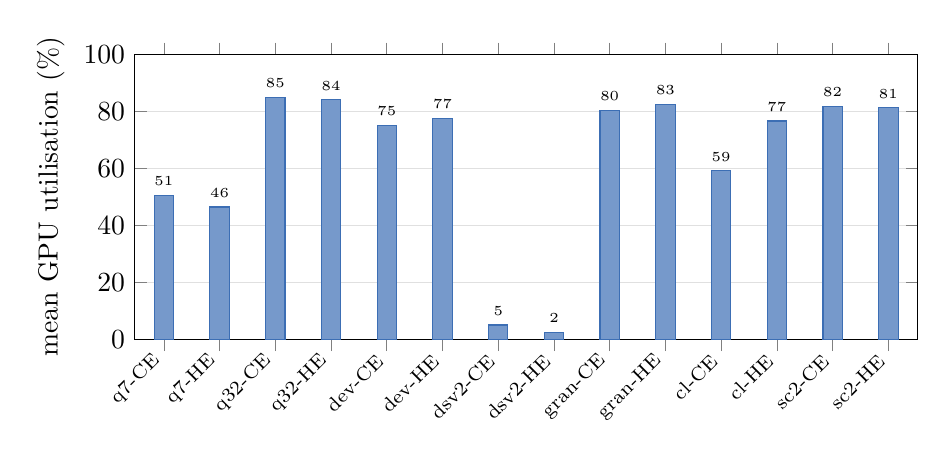
\begin{tikzpicture}
\begin{axis}[ybar, width=0.95\textwidth, height=5.2cm, bar width=7pt,
  ylabel={mean GPU utilisation (\%)}, ymin=0, ymax=100, enlarge x limits=0.04,
  symbolic x coords={q7-CE,q7-HE,q32-CE,q32-HE,dev-CE,dev-HE,dsv2-CE,dsv2-HE,gran-CE,gran-HE,cl-CE,cl-HE,sc2-CE,sc2-HE},
  xtick=data, x tick label style={rotate=45, anchor=east, font=\scriptsize},
  nodes near coords, nodes near coords style={font=\tiny}, every node near coord/.append style={/pgf/number format/fixed, /pgf/number format/precision=0},
  ymajorgrids, grid style={black!12}]
\addplot[fill=modelbar!70, draw=modelbar] coordinates {
  (q7-CE,50.5) (q7-HE,46.4) (q32-CE,84.9) (q32-HE,84.0) (dev-CE,75.0) (dev-HE,77.4)
  (dsv2-CE,5.0) (dsv2-HE,2.3) (gran-CE,80.2) (gran-HE,82.5) (cl-CE,59.1) (cl-HE,76.6) (sc2-CE,81.6) (sc2-HE,81.2)};
\end{axis}
\end{tikzpicture}
\caption{RQ3/RQ4. Mean GPU utilisation of the 14 matrix jobs of the full pilot
run (60\,s samples, 151--169 per job). q7/q32: Qwen2.5-Coder 7B/32B; dev:
Devstral 24B; dsv2: DeepSeek-Coder-V2 16B; gran: Granite-Code 20B; cl: Code
Llama 13B; sc2: StarCoder2 15B; CE: ClassEval; HE: HumanEval+.}
\label{fig:gpu}
\end{figure}

\paragraph{GPU use} Figure~\ref{fig:gpu} shows the mean GPU utilisation of the
14 matrix jobs. Twelve averaged 73\% (46--85\%) and were busy, meaning above
10\% utilisation, in 83--99\% of their samples. The 7B model's jobs sit lower,
at 46--51\%, because a small model leaves the GPU waiting on the harness's
CPU-side work such as sandboxed test execution. The two DeepSeek-Coder-V2 jobs
are outliers at 5.0\% and 2.3\%, with only 11--23\% busy samples
(Section~\ref{sec:res-rq4}).

\begin{tcolorbox}[enhanced, colback=modelbg, colframe=modelbar, boxrule=0.5pt, arc=1pt, left=6pt, right=6pt, top=3pt, bottom=3pt]
\small\textbf{Answer to RQ3.} Compiling the graph to arrays and dependencies
gave 2.0--2.7$\times$ speed-ups on 10-job smoke graphs and a mean concurrency
of 14.6 jobs on the 26-job study, under real fair-share contention. Twelve of 14
matrix jobs kept their GPU busy at a mean utilisation of 73\%.
\end{tcolorbox}

\subsection{RQ4: Observability and overhead}\label{sec:res-rq4}

\paragraph{What the scheduler does not show} In Slurm's view, all 14 matrix
jobs of the full run were equally healthy: RUNNING, within their limits, on
H100 nodes. The audit's GPU telemetry showed otherwise. Both DeepSeek-Coder-V2
jobs had used their GPUs at 2--5\% for more than 2.5 hours, while comparable
jobs ran at 75--85\%. The jobs were not failing and would have been reported
as successful. Without the audit, they would most likely have consumed their
full 24\,h allocation, plus requeues, at a fraction of the expected
throughput. With it, the anomaly is visible in one snapshot, and the
operator can inspect the inference server's log for that job, which the
pipeline keeps per job and per restart. The same telemetry gives the
calibration for the next sizing: for example, the parallel slots of the 7B
model could be raised.
The per-job server logs gave the cause when the study was moved to Narval
(A100 40\,GB), where the same model showed the same pattern. DeepSeek-Coder-V2
loaded fully onto the GPUs, but its generation requests stalled: they ended
with HTTP 500 at the inference server's 15-minute timeout after one output
token, and its server needed about 126--148\,GB of host memory, against
7--14\,GB for the other models (its first launch was killed by the 120\,GB
job memory limit). We could not make it complete the matrix and replaced it
with Gemma~3 27B in the study.

\paragraph{Overhead} Table~\ref{tab:micro} and Figure~\ref{fig:audit-scale}
report micro-benchmarks of the released template. Scaffolding takes 0.18\,s
and the full self-test (\V{1}--\V{6} on the full and smoke graphs, plus dry
runs) under 0.5\,s. The runner adds 7.1\,ms per executed step and 1.2\,ms per
skipped step. An audit snapshot takes 17\,ms for 10 cells and 0.52\,s for
5{,}000 cells, growing linearly. Collecting 100{,}000 JSON-lines records into
CSVs, grouped summaries and tables takes 1.4\,s. These costs are negligible
against GPU jobs measured in hours, and small enough for the login node, where
the audit runs.

\begin{table}[t]
\centering\small
\caption{RQ4. Overhead of the released template (login node, median of runs).}\label{tab:micro}
\begin{tabular}{@{}l l r@{}}
\toprule
Operation & Size & Time \\
\midrule
Scaffold \code{hpc/} into a repository & 18 files & 0.18\,s \\
Self-test (\V{1}--\V{6}, full + smoke graph, dry runs) & 4 stages, 10 + 6 cells & 0.48\,s \\
Runner overhead per executed step & 50 steps & 7.1\,ms \\
Runner overhead per skipped (resumed) step & 50 steps & 1.2\,ms \\
Audit snapshot & 10 / 100 / 1{,}000 / 5{,}000 cells & 0.02 / 0.03 / 0.12 / 0.52\,s \\
Collect (tables, summaries, md/tex) & 10{,}000 / 100{,}000 records & 0.17 / 1.41\,s \\
\bottomrule
\end{tabular}
\end{table}

\begin{figure}[t]
\centering
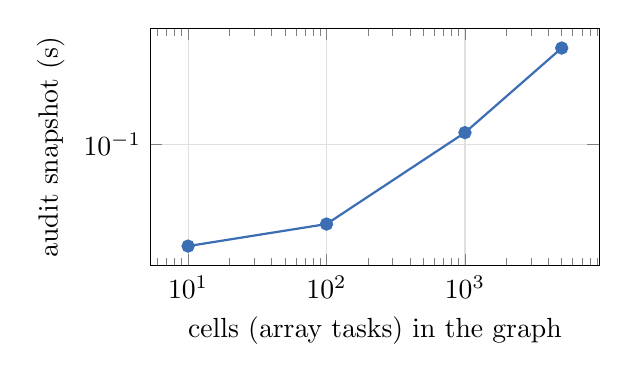
\begin{tikzpicture}
\begin{axis}[xmode=log, ymode=log, width=0.6\textwidth, height=4.6cm,
  xlabel={cells (array tasks) in the graph}, ylabel={audit snapshot (s)},
  ymajorgrids, xmajorgrids, grid style={black!12}, log basis x=10]
\addplot[mark=*, thick, color=modelbar] coordinates {(10,0.0174) (100,0.0254) (1000,0.1220) (5000,0.5210)};
\end{axis}
\end{tikzpicture}
\caption{RQ4. Audit latency against graph size: linear, and half a second at
5{,}000 cells.}
\label{fig:audit-scale}
\end{figure}

\begin{tcolorbox}[enhanced, colback=modelbg, colframe=modelbar, boxrule=0.5pt, arc=1pt, left=6pt, right=6pt, top=3pt, bottom=3pt]
\small\textbf{Answer to RQ4.} The audit exposed two silently under-utilised
GPU jobs that the scheduler reported as healthy. The machinery costs
milliseconds per step and under a second per audit or collection.
\end{tcolorbox}

\subsection{RQ5: Generality across repositories (pre-registered)}\label{sec:res-rq5}

The pilot shows that the approach works for one demanding paper, built by its
authors. RQ5 asks whether \skill{}, used by an agent, builds working pipelines
for \emph{independent} repositories.

\paragraph{Subjects} We will sample research repositories from GitHub with
these properties:
\begin{itemize}[leftmargin=1.4em, itemsep=1pt]
\item an associated paper with an experimental section;
\item a permissive licence;
\item Python entry points;
\item GPU-bound experiments;
\item at least two experimental factors.
\end{itemize}
Sampling is stratified over four domains: LLM evaluation, vision training,
graph learning, and software-engineering studies. Repositories whose
experiments need more than a fixed GPU budget per smoke run are excluded
\emph{before} running anything.

\paragraph{Procedure} For each repository, a fresh agent session with \skill{}
receives only the repository and the paper. It must reach a successful smoke
run. The full run is executed when its estimated cost fits the budget. A human
rater checks the coverage matrix against the paper.

\paragraph{Measures}
\begin{itemize}[leftmargin=1.4em, itemsep=1pt]
\item \emph{coverage}: the share of the paper's claims with a producing step;
\item \emph{smoke success} and the number of agent iterations to reach it;
\item \emph{source edits} in lines changed, and their kind;
\item \emph{human interventions};
\item \emph{guard events}: validator diagnostics, contract failures, gate
cancellations;
\item for full runs: makespan, concurrency, GPU utilisation, and agreement of
the collected results with the paper's reported numbers within the paper's
own uncertainty.
\end{itemize}
A baseline condition gives the same agent the same task \emph{without} the
skill. Its scripts are run under the same budget, and their failures,
completeness and login-node load are compared.

\begin{table}[t]
\centering\small
\caption{RQ5. Multi-repository study (pre-registered; results pending). One
row per repository; ``--'' marks values not yet measured.}\label{tab:repos}
\begin{tabular}{@{}l l r r r r r@{}}
\toprule
Repository & Domain & Claims & Covered & Smoke ok & Edits (LoC) & Interventions \\
\midrule
R1 & LLM evaluation & -- & -- & -- & -- & -- \\
R2 & vision training & -- & -- & -- & -- & -- \\
R3 & graph learning & -- & -- & -- & -- & -- \\
R4 & SE study & -- & -- & -- & -- & -- \\
\midrule
\multicolumn{7}{@{}l}{\emph{Baseline (agent without \skill{}) on the same repositories: pending.}} \\
\bottomrule
\end{tabular}
\end{table}

% =========================================================================
\section{Discussion}\label{sec:discussion}

\paragraph{Why programs, not prompts} Every protection in \cj{} that worked in
the pilot was a program: the gate, the dependency semantics, the contract
checks, the GPU guard and the telemetry. None was an instruction to the agent.
Instructions shape what the agent proposes. Programs decide what runs. We
believe this division is what makes agent-built experimental pipelines
acceptable on shared infrastructure. A mistaken agent produces a diagnostic
rather than an incident.

\paragraph{Smoke runs are tests of the experiment} Software engineers would not
ship code whose every module had never been executed. Yet large experiments are
routinely launched whose analysis stage has never run. The smoke projection
makes structural coverage of the apparatus a precondition of the real run, at
about one GPU-hour in the pilot.

\paragraph{Authenticity as traceability} An ``authentic'' result is one that a
reader can trace: from the sentence in the paper, through the coverage matrix,
to the collected CSV, the step that wrote it, the job that ran the step, the
node and GPU it ran on, and the commit and configuration it used. \cj{}
produces every link of this chain as a by-product of execution. It does not
guarantee that a result is \emph{correct}: a wrong metric implementation runs
just as smoothly as a right one.

\paragraph{Telemetry is a scientific instrument} The under-utilised jobs of
RQ4 would not have changed a single number of the study. They would have
changed its cost and duration, and they hint at a configuration problem that a
reviewer of the study would want to know about. Recording resource use next to
results turns ``it ran'' into ``it ran as designed''.

% =========================================================================
\section{Threats to Validity}\label{sec:threats}

\paragraph{Construct validity} Speed-up is measured against the sum of job run
times, not against a hand-written pipeline for the same study. Queue waits
depend on fair-share and cluster load at the time of the runs, which we did not
control. GPU utilisation from \code{nvidia-smi} is a coarse proxy for useful
work.

\paragraph{Internal validity} The pilot pipeline was written by the authors of
the \auto{} paper. It is the prototype of the template, not an output of the
skill used by an independent agent session. RQ5 is designed to remove this
threat. The full-run figures are a snapshot taken during the run; final totals
will differ. The contract and guard tests of RQ2 were constructed by us.

\paragraph{External validity} One paper, one cluster and one scheduler.
Other Slurm sites need different GPU names, module stacks and environment
recipes. Other schedulers (PBS, LSF) need a different submitter and audit
backend. Studies whose unit of work is a multi-node training job exercise
\code{srun} launching and the node check, which the pilot did not.

\paragraph{Conclusion validity} The pilot gives descriptive evidence (counts,
times, utilisation), not statistical comparisons. RQ5 is pre-registered so that
its comparison with the baseline is not shaped by the results.

% =========================================================================
\section{Conclusion}\label{sec:conclusion}

\cj{} treats every claim of a paper as a job and every job as something a
program checks. An agent proposes the experiment graph. A validator, the
scheduler's dependency semantics, data contracts and runtime guards decide what
runs. A live audit and a collector report what happened, down to the GPU
utilisation of each job and up to the coverage of each claim. In a pilot that
runs a 44{,}352-run software-engineering evaluation on H100 nodes:
\begin{itemize}[leftmargin=1.4em, itemsep=1pt]
\item smoke projections covered every stage in about 20 minutes;
\item failed gates cancelled 75 dependent jobs before they cost anything;
\item the full study ran at a mean concurrency of 14.6 jobs;
\item the audit caught two silently idle GPU jobs.
\end{itemize}
The method ships as \skill{}, an agent skill that installs with one command. A
pre-registered study on independent repositories will show how far it
carries.

\section*{Data Availability}\label{sec:data}

The \skill{} skill, its template and installation instructions are public at
\url{https://github.com/ai4se4ai-lab/use-hpc-claude-skill}. The pilot
pipeline, its run ledgers, the \code{sacct} extract, the GPU telemetry
summaries and the analysis script (\code{docs/use-hpc-eval/}) are in the
\auto{} replication package.
% TODO(author): add DOI of the archived package.

\section*{Declarations}

\textbf{Funding.} [To be completed.]
\textbf{Conflict of interest.} The author declares no conflict of interest.
\textbf{Use of generative AI.} The approach studied here uses an LLM agent
(Claude Code) to configure experiment pipelines, and an LLM assistant was used
in preparing this manuscript. Its use is [to be declared according to the
journal's policy]. All reported numbers were produced by the scripts named in
the text from logged data.

\bibliography{use-hpc-references}

\end{document}
